% 
% Aprendizado de máquina
%

\newcommand{\vect}[1]{\mathbf{#1}}
\newcommand{\norma}[1]{\lVert #1 \rVert}

% Usar Inductive Principles for Learning from Data como referência "dos
% tópicos" para esse assunto, e também o "Uma Introdução às Support Vector
% Machines".
% Tomar cuidado em manter a consistência entre as diferentes notações
% usadas entre as referências.
%
% - A teoria do aprendizado estatístico
% - Métodos paramétricos
% - Métodos adaptativos
% - Risco esperado, risco estatístico
% - Classificação binária
% - Classificação multi-classes
% - Como adaptar um classificador binário para um problema multi-classes
%   (Pairwise, e esqueciooutro)
%
% Apresentar (brevemente) algumas outras técnicas também:
% (lista baseada em wiki/Supervised_learning#Approaches_and_algorithms)
% - redes neurais artificiais
% - inferência bayesiana
% - ...
%
% FIXME Aqui realmente estou em dúvida. Devemos apresentar TODAS as
% técnicas, uma por parágrafo, ou apresentar uma a uma?
% -- Pelo que tenho visto em outras monografias, não é necessário
%  apresentar o estado da arte da área de aprendizado (Ver Trabalhos
%  Relacionados no Google Docs)

Um dos comportamentos mais característicos de sistemas computacionais que possam ser considerados inteligentes é o de melhorar o seu desempenho para resolver algum problema quando este se depara com a mesma situação por mais de uma vez ~\cite{luger2004inteligencia}. ~\apudonline{simon1983should}{luger2004inteligencia} define o conceito de aprendizado de máquina afirmando que qualquer mudança que melhore o seu desempenho na segunda vez que ele repetir a mesma tarefa, ou numa tarefa da mesma população.

Nem sempre é possível obter um resultado ótimo para novas situações, pois na maioria dos casos não é possível apresentar a um sistema a quantidade de exemplos (ou experiências anteriores) necessárias para representar todos os casos possíveis. Por isso, as técnicas de aprendizado fazem uso da inferência indutiva, que consiste em prever novas situações baseando-se em um conjunto particular de exemplos~\cite{luger2004inteligencia}.

A construção da hipótese no aprendizado indutivo ocorre por meio da exposição de exemplos ao algoritmo de indução, e este processo é chamado de \emph{treinamento}. O processo de atribuir rótulos ou classes a novos exemplos é chamado de \emph{classificação}.

Porém, se o conjunto de exemplos usado para a indução for muito pequeno ou pouco representativo, há o risco de que as hipóteses escolhidas não descrevam corretamente novas situações e o sistema inteligente traga resultados incorretos~\cite[p. 90]{rezende2003sistemas}.

Sistemas de aprendizado de máquina podem ser divididos em dois tipos de acordo com a maneira que é feito o treinamento: supervisionados e não-supervisionados.

O aprendizado supervisionado é aquele em que há exemplos pré-existentes e estes já possuem rótulos. Estes rótulos podem ter sido atribuídos por um especialista no domínio ou representam resultados de experiências anteriores do sistema. Um classificador baseado em aprendizado supervisionado deve tentar estabelecer uma hipótese que seja genérica a ponto de que o algoritmo possa classificar corretamente novos casos. Uma hipótese muito genérica pode resultar em uma classificação inadequada (\emph{underfitting} --- sub-ajuste), ao passo que uma hipótese que descreva corretamente apenas os exemplos que foram usados para o treinamento pode ter um desempenho inadequado em casos novos (\emph{overfitting} --- sobre-ajuste).

No aprendizado não-supervisionado, não há rótulos para atribuir aos exemplos, pois o objetivo do algoritmo é encontrar grupos de exemplos que possuam semelhança entre eles. As técnicas deste modelo são referenciadas como sendo \emph{técnicas de agrupamento} ou \emph{clustering}~\cite{rezende2003sistemas}.
%FIXME terminar não-supervisionado (dar uma olhada no livro do Luger)

\subsection{Técnicas de aprendizado supervisionado}

Dentre as técnicas de aprendizado supervisionado mais populares estão Redes Neurais, Máquinas de Vetores de Suporte (\emph{Support Vector Machines} --- SVMs), $k$ Vizinhos Mais Próximos ($k$-NN) e \emph{Naïve Bayes}.

% FIXME faltou descrever GGM, RBF, Redes Bayesianas e árvores de decisão

O $k$-NN é um algoritmo de aprendizado supervisionado que requer pouco esforço durante a etapa de treinamento, porém a classificação acaba tendo um custo alto, no pior caso, o novo exemplo tem que ser comparado com todos os vizinhos. Para classificar um novo elemento se busca os $k$ vizinhos rotulados mais próximos do novo elemento através de uma medida de similaridade, como medida euclidiana \cite{ferrero-algoritmo} para conjuntos numéricos e medida do cosseno \cite{tan2006effective} na classificação de textos.

A técnica de \emph{Árvores de Decisão} utilizam o aprendizado não-incremental, onde o algoritmo induz um conjunto de exemplos a uma árvore construída da raiz para as folhas, não importando a ordem em que se apresentam os exemplos. Os nós das árvores são os atributos, onde contém também os testes binários ou multivalorados, e os ramos valores para esses atributos~\cite{de-categorizacao}.

\emph{Naïve Bayes} é um algoritmo de aprendizado supervisionado, que
utiliza probabilidade para a classificação e supõe que as variáveis de cada
exemplo são condicionalmente independentes \cite{de-categorizacao}, as
probabilidades são calculadas de acordo com o Teorema de Bayes
\cite{kim2003poisson}, para a classificação de um elemento desconhecido, é
calculada a probabilidade de todas as classes e a classe com maior
probabilidade é escolhida como rótulo para o elemento desconhecido.
~\cite{pardo2002aprendizado}

As \emph{Redes Neurais Artificiais} (RNAs) são modelos matemáticos baseados no neurônio biológico, têm a capacidade computacional adquirida por meio de aprendizado e generalização, são capazes de resolver problemas de aproximação, predição, classificação e otimização. A aprendizagem de uma rede neural ocorre a partir dos exemplos e tende a melhorar seu desempenho conforme a qualidade dos exemplos, já a generalização surge como consequência do aprendizado. O processamento das informações pode ser feito de forma paralela e distribuída, através dos neurônios da rede neural artificial, onde cada neurônio é um elemento processador.~\cite{rezende2003sistemas}

\emph{Support Vector Machines} é uma técnica modelada como um problema de otimização que tenta encontrar, no espaço do conjunto de exemplos, um hiperplano que separe com maior margem os exemplos de cada uma das duas classes. Em razão da aplicação desta técnica em parte da metodologia proposta neste trabalho, será feita uma apresentação mais detalhada a partir da seção \ref{sec:svm}) (página \pageref{sec:svm}). Antes disso, as seções a seguir buscam apresentar os conceitos e terminologia comumente utilizados na apresentação das SVMs.

\subsection{Formalização do aprendizado supervisionado}

Como já brevemente apresentado, no problema de aprendizado supervisionado existe a figura de um professor que indica qual é o rótulo correto para cada exemplo \apud{haykin1994neural}{lorena2003introducaoas}. Sendo assim, cada exemplo pode ser descrito na forma $(\vect{x}_i, y_i)$, aonde $\vect{x}_i$ denota um exemplo e $y_i$ seria a classe ou rótulo. Também, após o processo de treinamento, pode-se descrever o classificador como uma função $f(\vect{x}) = y$, sendo que $\vect{x}$ não é necessariamente um dos valores de $\vect{x}_i$.

Os valores dos rótulos que os exemplos podem assumir podem ser discretos ou contínuos. Para o caso dos contínuos assume-se que é possível obter $1,\dotsc,k$ valores. Quando $k = 2$, o problema é denominado como sendo de \emph{classificação binária}. Quando $k > 2$ denomina-se como sendo um problemas de \emph{classificação multiclasses}.

Os exemplos $\vect{x}_i$, são representados por vetores com as \emph{características} (também denominadas \emph{atributos}) de cada exemplo. Cada exemplo $\vect{x}_i$ possui $m$ atributos e também pode ser representado como $\vect{x}_i = (x_{i1},\dotsc,x_{im})$. Os atributos podem assumir dois tipos de valores: nominais ou contínuos. Os atributos nominais assumem valores que não possuem ordem entre si e sua representação tem função simbólica (por exemplo: segunda-feira, azul, não). Os atributos contínuos possuem ordem entre si e comumente representam valores dos domínios $\mathbb{Z}$ e $\Re$.

O objetivo de uma técnica de aprendizado de máquina é obter uma função $f(\vect{x}) = y$ que obtenha um $y$ adequado aos exemplos que foram apresentados pelo \emph{professor} por meio de indução~\cite{osuna1997support}.

% parece ser muito pouco conteúdo, porém mais detalhes como (overfitting) ou
% (como avaliar o desempenho de alguma técnica de AM) já foram (acima) ou serão
% (em classificação de textos).

% latex não sabe deixar o í maiúsculo, então...
\subsection{Aprendizado estatístico}\label{sec:aprendizado}

Sendo $f$ um classificador e $F$ o conjunto dos classificadores possíveis gerados pelo algoritmo de aprendizado, pode-se descrever o aprendizado como a busca por um classificador $\hat{f}$ que melhor aproxime os resultados aos dos exemplos $T$. Para descobrir qual é o melhor classificador do conjunto $F$, utiliza-se uma \emph{medida de discrepância} ou perda, que indica o quanto de erro houve com um classificador $f$ em relação aos exemplos conhecidos \cite{vapnik1998statistical}. Para problemas de classificação binária, emprega-se a função de custo descrita na equação \ref{eq:custo_binario}, que retorna $1$ quando classificado corretamente e $0$ quando erra.
\begin{equation}\label{eq:custo_binario}
  c(f(\vect{x}), y) = \frac{1}{2} | y - f(\vect{x})|
\end{equation}

Quando a distribuição $P(\vect{x},y)$ é conhecida, pode-se calcular o risco esperado de um classificador com a equação \ref{eq:risco_funcional}. Porém, como a distribuição dos exemplos não é conhecida, é necessário induzir um classificador $\hat{f}$ a partir dos exemplos disponíveis de maneira que seja possível diminuir o erro sobre os dados \cite{scholkopf2002learning}. 
\begin{equation}\label{eq:risco_funcional}
  R(f) = \int{ c(f(\vect{x})dP(\vect{x}, y) }
\end{equation}

É possível medir o risco do classificador $\hat{f}$ avaliando-se o \emph{risco empírico}, que é descrito na equação \ref{eq:risco_empirico}.
\begin{equation}\label{eq:risco_empirico}
  R_{emp}(f) = \frac{1}{n}\sum_{i=1}^n{c(f(\vect{x}_i),y_i)}
\end{equation}

A partir da lei dos grandes números, pode-se observar que o risco empírico aproxima-se do risco esperado quando o número de amostras tende para infinito \apud{vapnik1998statistical}{osuna1997support}. Porém, para exemplos pequenos não é possível garantir que o risco empírico aproxime-se do risco esperado. \citeonline{lorena2003introducaoas} exemplifica esta situa\c{c}ão com o caso de um classificador que aprende um conjunto de exemplos mas classifica casos novos aleatoriamente, no qual o risco empírico seria 0, mas o risco esperado seria 0,5. Além disso, a simples minimizac\c{c}ão do risco empírico não é ideal para um algoritmo de aprendizado porque o classificador resultante poderia estar sobreajustado ao conjunto de exemplos.

Com o objetivo de dificultar a possibilidade de que haja sobreajuste do classificador, \citeonline{vapnik2000nature} define um limite no risco empírico baseado na complexidade do conjunto de fun\c{c}ões de classificadores $F$. A inequa\c{c}ão \ref{eq:minrisco} apresenta este limite, aonde o risco empírico está associado também há um \emph{termo de capacidade} e, aonde $h$ representa a complexidade do conjunto de classificadores que está sendo avaliado.
\begin{equation}\label{eq:minrisco}
  R(f) \leqslant R_{emp}(f) + \sqrt{\frac{h(\ln(\frac{2n}{h})+1)-\ln(\frac{\phi}{4})}{n}}
\end{equation}

Essa medida $h$, é conhecida também como \emph{dimensão VC} (de Vapnik-Chervonenkis) e representa a quantidade de exemplos do treinamento que podem ser separados com um determinado conjunto de fun\c{c}ões classificadoras de $F$. Estes conjuntos $F_k$ são subconjuntos de $F$ e são ordenados de acordo com seus valores de $k$, de maneira que podem ser representados na forma $F_0\subset F_1 \subset \dotsb \subset F_q \subset F$.

Como o risco empírico diminui à medida que o valor de $h$ aumenta, pode-se com isso encontrar um valor ótimo, ou em outras palavras um conjunto $F_k$, que represente um compromisso aceitável entre o valor do risco empírico (sendo este sempre o menor dentre todas as fun\c{c}ões de $F_k$) e a complexidade da fun\c{c}ão que representa o classificador. Porém, o cálculo da dimensão VC nem sempre é definido ou seu valor é infinito. A escolha da melhor fun\c{c}ão de $F_k$ representa o principal conceito da \emph{mimiza\c{c}ão do risco empírico} \apud{muller2001introduction}{lorena2003introducaoas}. A figura \ref{fig:minimizacao} apresenta este conceito.

\begin{figure}[h!]
  \centering
  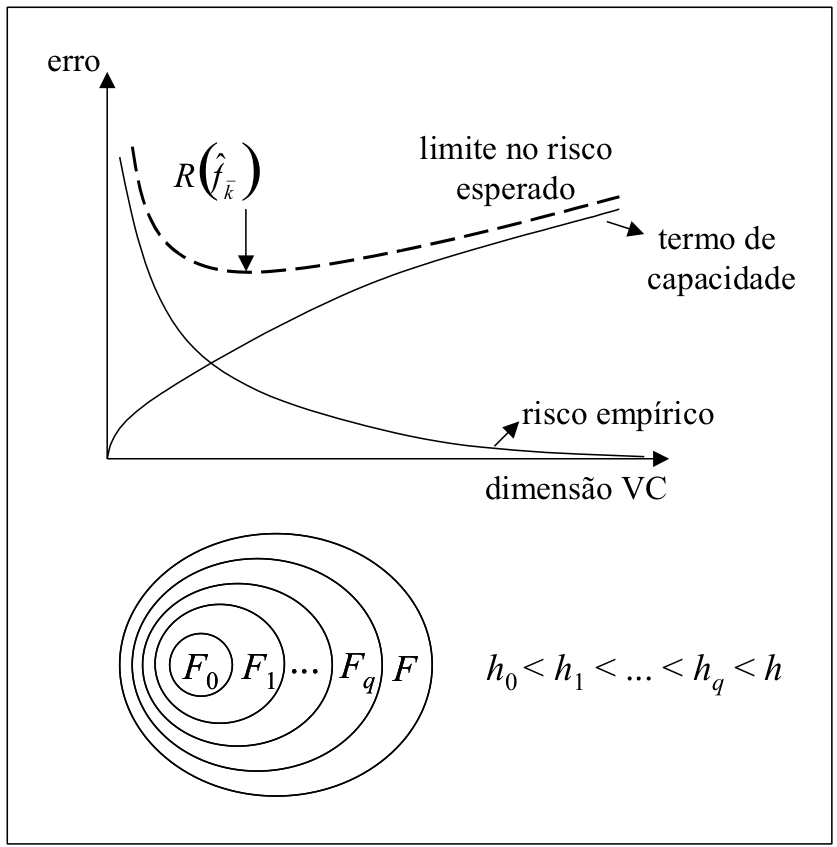
\includegraphics[width=0.5\textwidth]{img/fig-minimizacao.png}
  \figinfox{Princípio da minimização do risco estrutural e dimensões VC}{LORENA, 2003}
  \label{fig:minimizacao}
\end{figure}

Para o caso de classificadores lineares $f(\vect{x}) = \vect{x}\cdot\vect{w} + b$, é possível melhorar a qualidade da classifica\c{c}ão introduzindo o conceito de \emph{margem} entre os exemplos e o hiperplano separador definido por $f(x)$ \cite{smola2000advances}. Para o caso de problemas binários com classifica\c{c}ão $y_i$ sendo $y_i \in {-1, +1}$, é possível definir esta margem (que é negativa em caso de classifica\c{c}ão incorreta, por meio da defini\c{c}ão de $\varrho(f(\vect{x}_i,y_i))$ na equa\c{c}ão \ref{eq:margemlinear}.
\begin{equation}\label{eq:margemlinear}
  \varrho(f(\vect{x}_i),y_i) = y_i f(\vect{x}_i)
\end{equation}

Sendo que $I(q) = 1$ se $q$ é verdadeiro e $I(q) = 0$ se $q$ é falso.

Tendo a defini\c{c}ão de erro de classifica\c{c}ão baseado em uma margem até o hiperplano separado, é possível então estabelecer uma medida para a qualidade da separa\c{c}ão de um dado classificador $f(\vect{x})$ por meio da equa\c{c}ão \ref{eq:errorho}.
\begin{equation}\label{eq:errorho}
  R_\rho(f) = \frac{1}{n}\sum^{n}_{i=1}{I(y_i f(\vect{x}_i) < \rho))}
\end{equation}

Com isso, é possível estabelecer o limite descrito pela equa\c{c}ão \ref{eq:riscoestrutural}. Nela, tem-se $c$ com probabilidade $1 - \theta \in [0,1]$, para $\rho > 0$ e $F$ sendo uma fun\c{c}ão linear, com $\norma{\vect{x}} \le R$ e $\norma{\vect{w}} \le 1$. Esse limite constitui a \emph{minimiza\c{c}ão do risco estrutural}, introduzido por \cite{vapnik1998statistical}.
\begin{equation}\label{eq:riscoestrutural}
  R(f) \leqslant R_\rho(f) + \sqrt{
        \frac{c}{n}
        \left(
          \frac{R^2}{\rho^2}
          \log^2\left(\frac{n}{\rho}\right) +
          \log\left(\frac{1}{\theta}\right) \right)
       }%sqrt
\end{equation}

% FIXME adicionar alguma conclusão aqui amarrando tudo, algoc como: assim, o conceito de minimização do risco estrutural demonstra uma maneira de melhorar a capacidade de generalização de um algoritmo de aprendizado.

\subsection{Support Vector Machines --- \it{SVMs}}\label{sec:svm}
%
%   - problema primal
%   - problema dual (e teoria "dos lagrangianos")
%   - vetores de suporte
%   - SVM com margens rígidas
%   - SVM com margens flexíveis (E_i)
%   - kernels (RBF gaussiano etc)

A técnica de aprendizado de máquina supervisionado conhecida como \emph{Support Vector Machine} (SVM), ou \emph{Máquinas de Vetores de Suporte} foi introduzida por Boser, Guyon e Vapnik em 1992 com a publica\c{c}ão de \emph{A training algorithm for optimal margin classifiers}\nocite{boser1992training}. Esta baseia-se no trabalho da teoria do aprendizado estatístico desenvolvida por Vapnik et al. desde a década de 1960.

SVMs usam o princípio de que quanto mais largas as margens de um hiperplano separador de uma fun\c{c}ão, que foi explicado na se\c{c}ão \ref{sec:aprendizado} por meio do conceito de minimiza\c{c}ão do risco estrutural, maiores são as chances de que ele possa prover uma boa generaliza\c{c}ão dos dados que estão sendo usados como exemplo \cite{chapelle2002choosing}. Então, SVMs buscam encontrar um hiperplano descrito por $f(\vect{x}) = \vect{w}\cdot\vect{x} + b = 0$ que tenha maior margem entre as classes e menor complexidade estrutural por meio da resolu\c{c}ão de um problema de otimiza\c{c}ão.

Para encontrar o hiperplano separador ideal, é necessário utilizar (pelo menos) dois pontos do conjunto de exemplos. Sejam $\vect{x}_1$ e $\vect{x}_2$ dois exemplos do conjunto de treinamento $T$ que possui um conjunto de exemplos $X$ com rótulos do conjunto de exemplos $Y = \{-1, +1\}$, e cada um deles fica em um lado diferente do hiperplano separador. Para encontrar o hiperplano separador $f(\vect{x}) = \vect{w}\cdot\vect{x} + b = 0$ entre $\vect{x}_1$ e $\vect{x}_2$, é necessário conhecer o vetor $\vect{w}$, que deve ser normal a este hiperplano e que é usado para calcular o tamanho da margem.

\begin{figure}[h!]
  \centering
  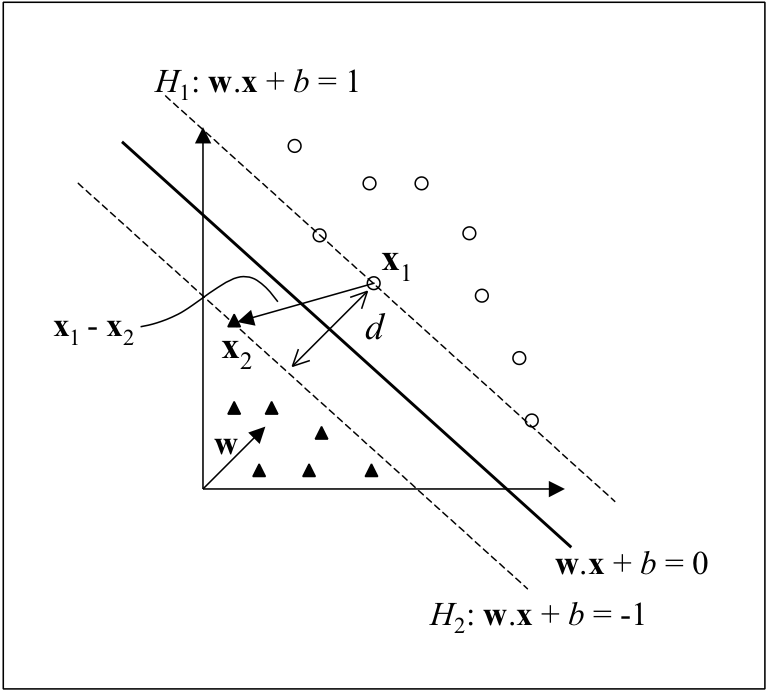
\includegraphics[width=0.5\textwidth]{img/fig-hiperplanos.png}
  \figinfo{Hiperplano separador e margens}{LORENA, 2003}
  \label{fig:hiperplanos}
\end{figure}

Como um dos objetivos do problema de otimização é obter uma margem larga entre os exemplos, pode-se restringir a busca por $\vect{w}$ apenas em termos do cálculo do tamanho da margem. Para isso, é necessário calcular a distância entre dois hiperplanos que são formados pelos exemplos $\vect{x}_1$ e $\vect{x}_2$. Sejam $H_1: \vect{w}\cdot\vect{x} + b = +1$ e $H2: \vect{w}\cdot\vect{x} +b = -1$ dois hiperplanos que ficam paralelamente acima e abaixo, respectivamente, do hiperplano separador. Além disso, assume-se que $H_1$ passa por $\vect{x}_1$ e $H_2$ passa por $\vect{x}_2$. A figura \ref{fig:hiperplanos} mostra a relação entre os hiperplanos e os pontos $\vect{x}_1$ e $\vect{x}_2$.

Conhecendo os hiperplanos, agora é possível calcular a distância entre os hiperplanos que servem de fronteira entre cada ponta da margem do hiperplano separador. A equação \ref{eq:projecao_w} apresenta o cálculo necessário para projetar $\vect{x}_1 - \vect{x}_2$ na direção de $\vect{w}$, que é perpendicular ao hiperplano separador $\vect{w}\cdot\vect{x} + b = 0$.
\begin{equation}\label{eq:projecao_w}
  (x_1 - x_2)
    \left(
      \frac{ \vect{w} }{ \norma{\vect{w}} }
      \cdot
      \frac{(x_1 - x_2)}{ \norma{\vect{x}_1 - \vect{x}_2} }
    \right)
\end{equation}

Sabendo que $\vect{w}\cdot\vect{x}_1 + b = +1$ e $\vect{w}\cdot\vect{x}_2 + b = -1$, e levando em conta que deseja-se saber o comprimento do vetor resultante, é usada a norma da equação \ref{eq:projecao_w} para chegar à equação \ref{eq:projecao_w2}, que indica a distância $d$ utilizada na figura \ref{fig:hiperplanos}:
\begin{equation}\label{eq:projecao_w2}
  \frac{2}{\norma{\vect{w}}}
\end{equation}

Portanto, as distâncias entre $\vect{x}_1$, $\vect{x}_2$ e o hiperplano separador $\vect{w}\cdot\vect{x} + b = 0$ são $\frac{1}{\norma{\vect{w}}}$, e com isso, é possível definir o problema de otimização como definido pelo problema de otimização \ref{eq:max_w0}. A restrição \ref{eq:max_w1} indica que $H_1$ e $H_2$ devem passar, respectivamente, pelos vetores $\vect{x}_1$ e $\vect{x}_2$.
\begin{eqnarray}
& \label{eq:max_w0}\operatorname{Maximizar} & \frac{2}{\norma{\vect{w}}} \\
& \label{eq:max_w1} \operatorname{sujeito\;a} & y_i(\vect{w}\cdot\vect{x}_i + b) - 1 \ge 0 \quad i = 1,\dotsc,n.
\end{eqnarray}

No problema de maximização \ref{eq:max_w0}, $\frac{2}{\norma{\vect{w}}}$ pode também ser descrito como um problema de minimização de $\norma{\vect{w}}^2/{2}$:
\begin{eqnarray}
& \label{eq:min_w0}\operatorname{Minimizar} & \frac{\norma{\vect{w}}^2}{2} \\
& \nonumber \operatorname{sujeito\;a} & y_i(\vect{w}\cdot\vect{x}_i + b) - 1 \ge 0 \quad i = 1,\dotsc,n.
\end{eqnarray}

A partir deste ponto, o problema \ref{eq:min_w0} pode ser resolvido com técnicas de programação quadrática (PQ) \cite{osuna1997support}. Este tipo de problema pode ser solucionado utilizando uma função Lagrangiana e adicionando as restrições à função objetivo junto com os multiplicadores de Lagrange $\alpha_i$ \cite{smola2000advances}. A equação \ref{eq:lagrange0} deve ser minimizada, o que significa maximizar $\alpha_i$ e minimizar $\vect{w}$ e $b$. O problema é representado desta forma para que a restrição \ref{eq:max_w1} possa ser representada na forma dos multiplicadores $\alpha_i$, o que facilita os cálculos mais adiante, e também porque os dados de treinamento apenas aparecem na forma de produtos entre vetores \cite{burges1998tutorial}, o que permite o uso de \emph{kernels}, que são apresentados na seção \ref{sec:naolinear}.
\begin{equation}\label{eq:lagrange0}
  L(\vect{w}, b, \vect{\alpha}) = \frac{1}{2}\norma{\vect{w}}^2 - 
       \sum_{i=1}^n{\alpha_i(y_i(\vect{w}\cdot\vect{x}_i + b) - 1)}
\end{equation}

Tem-se ponto de sela, então:
\begin{eqnarray}\label{eq:sela}
  \frac{\partial{L}}{\partial{b}} = 0 & \text{e} & \frac{\partial{L}}{\partial{\vect{w}}} = 0
\end{eqnarray}
E com isso:
\begin{eqnarray}
&  \label{eq:lagsum0}  \sum_{i=1}^n{\alpha_i y_i} = 0 \\
&  \label{eq:lagsum1}  \vect{w} = \sum_{i=1}^n{\alpha_i y_i\vect{x}_i}
\end{eqnarray}

Assim, substituindo equações \ref{eq:lagsum0} e \ref{eq:lagsum1}, é possível formular o problema de otimização:
\begin{eqnarray}\label{eq:maxalpha}
\begin{array}{rl}
   %\operatorname*{Maximizar}_{\alpha}
   \underset{\alpha}{\operatorname{Maximizar}}
   & \sum_{i=1}^n{\alpha_i - \frac{1}{2}}
                            \sum_{i,j=1}^n{\alpha_i\alpha_j y_i y_j(\vect{x}_i\cdot\vect{x}_j)} \\
\operatorname{sujeito\;a} &
  \begin{cases}
    \alpha_i \geqslant 0, \forall{i} = 1,\dotsc,n \\
    \sum_{i=1}^n{\alpha_i y_i} = 0
  \end{cases}
\end{array}
\end{eqnarray}

A equação \ref{eq:maxalpha} é denominada a \emph{forma dual} do problema, ao passo que a formulação original na equação \ref{eq:min_w0} é denominada a \emph{forma primal}, baseada no trabalho de \apudonline{fletcher1987practical}{burges1998tutorial}.

É possível utilizar as condições KKT (de Karush-Kuhn-Tucker), descritas em \citeonline[proposição 3.3.1]{bertsekas-nonlinear}, visto que o problema de otimização \ref{eq:maxalpha} possui restrições lineares e a função objetivo é convexa \cite{burges1998tutorial}. Assim, segundo essas condições, é possível encontrar $\vect{w^*}$ e $b^*$ que podem ser considerados solução ótima para o problema a partir da solução do problema dual ao encontrar $\alpha_i^*$:
\begin{equation}\label{eq:dualalpha}
  \alpha_i^*(y_i(\vect{w^*}\cdot\vect{x}_i+b^*) - 1) = 0, \forall{i}=1,\dotsc,n
\end{equation}

Nesta equação $\alpha_i^*$ é diferente de zero apenas para os valores que tocam a borda das margens do hiperplano de decisão ($H_1$ e $H_2$). Assim, esses dados são chamados de \emph{vetores de suporte}, pois são os dados mais significativos para a localização de hiperplano $\vect{w}\cdot\vect{x} + b = 0$.

E para calcular $b^*$, de acordo com \ref{eq:dualalpha}:
\begin{equation}\nonumber
  b^* = \frac{1}{n_{SV}}\sum_{x_j \in SV}{\frac{1}{y_j} - \vect{w^*}\cdot\vect{x}_j}
\end{equation}

Aonde $n_{SV}$ é o número de vetores de suporte e $SV$ o conjunto dos mesmos.

% ALELUIA!!!!!!!!!!!! PQPQPQPQPQPQPQP!!!
Finalmente, obtém-se a seguinte função classificadora:
\begin{equation}\label{eq:classificadora}
  g(\vect{x}) = \operatorname{sinal}(f(\vect{x}))
              = \operatorname{sinal}\left(
                  \sum_{x_i \in SV}{y_i\alpha_i^*\vect{x}_i\cdot\vect{x}+b^*}
                \right)
\end{equation}

\subsubsection{Margens suaves}

% seção está incompleta, não explica bem como o erro é tratado em si

Para tratar os casos em que há \emph{outliers} nos exemplos, ou seja, dados que estão rotulados incorretamente ou com algum ruído, utiliza-se a técnica de margens suaves, que é uma saída mais simples que SVMs não-lineares \cite{burges1998tutorial}.

Utiliza-se variáveis de folga $\xi_i$ para cada exemplo $\vect{x}_i$ do conjunto de treinamento. Essas variáveis são adicionadas à restrição do problema primal:
\begin{equation}\label{eq:restrsuave}
  y_i(\vect{w}\cdot\vect{x}_i+b) \geqslant 1 - \xi_i,\quad\forall{i}=1,\dotsc,n
\end{equation}

Ao passo que a função objetivo é reformulada como:
\begin{equation}
  \underset{\vect{w}, b, \vect{\xi}}{\operatorname{Minimizar}}\quad
         \frac{1}{2}\norma{\vect{w}}^2+C\left(\sum_{i=1}^n{\xi_i}\right)
\end{equation}

A constante $C$ impõe uma penalização à violação das restrições \ref{eq:restrsuave} do problema de otimização. O valor desta constante é definida pelo usuário e sua definição depende de testes baseados no conjunto de treinamento. Algumas abordagens para a escolha deste parâmetro foram apresentadas por \citeonline{chapelle2002choosing}, \citeonline{cherkassky2004practical}, \citeonline{quang2002evolving} e \cite{ben2010user}.

% FIXME descrever o método de busca em grade de ben2010user, pois é o que
% usamos

\subsubsection{Classificação não-linear}\label{sec:naolinear}

Segundo o teorema de \citeonline{cover1965geometrical}, as chances de que um conjunto de exemplos não linearmente separável possa ser separado por um hiperplano é grande quando este é disposto em um espaço de maior dimensionalidade. Assim, a implementação das máquinas de vetores de suporte utiliza esta técnica para conseguir separar dados ainda de maneira \emph{linear} \cite{burges1998tutorial}.

Com isso, os dois vetores $\vect{x}$ e $\vect{x}_i$, que são utilizados na função de decisão \ref{eq:classificadora}, são convertidos para o espaço de maior dimensão por um mapeamento $\vect{\Phi}: X \rightarrow \Im$, aonde $X$ é o espaço de entrada e $\Im$ o \emph{espaço de características}.

Adicionalmente, o produto entre os vetores $\vect{x}$ e $\vect{x}_i$ é representado como uma função $K(\vect{x}_i, \vect{x}_j) = \vect{\Phi}(\vect{x}_i)\cdot\vect{\Phi}(\vect{x}_j)$. Esta função é chamada de \emph{função kernel} e tem por finalidade permitir o uso de funções que atentem às condições definidas pelo teorema de Mercer \cite[p. 141]{burges1998tutorial}. Esta forma de representação permite que use-se estas funções de kernel dentro da implementação de uma SVM sem a necessidade de conhecimento dos detalhes internos das mesmas. O quadro \ref{quadro:kernels} apresenta alguns dos kernels mais populares utilizados com SVMs~\cite{lorena2003introducaoas}.

\begin{table}
\centering
\begin{tabular}{|c|c|c|}
\hline
Tipo de kernel & Função & Parâmetros \\
\hline
Polinomial & $(\delta(\vect{x}_i\cdot\vect{x}_j)+\kappa)^d$ & $\delta$, $\kappa$, e $d$ \\
Gaussiano & $\exp(-\sigma\norma{\vect{x}_i-\vect{x}_j}^2)$ & $\sigma$ \\
Sigmoidal & $\tanh(\delta(\vect{x}_i\cdot\vect{x}_j)+\kappa)$ & $\delta$ e $\kappa$ \\
\hline
\end{tabular}
\quadro{Funções de kernel comumente usadas}\label{quadro:kernels}
\end{table}

\subsubsection{Classificação multiclasses}\label{sec:svmmulti}

% hsu2002comparison

Como SVMs fazem classificação binária, é necessário o uso de alguma técnica para adaptar problemas de classificação multiclasses. As mais populares são \emph{um contra todos} (\emph{one-against-all}) e \emph{um contra um} (\emph{one-against-one}).

Na técnica \emph{um contra todos}, é treinada uma SVM para cada classe contra todas as outra classes ao mesmo tempo. \citeonline{vapnik1998statistical} propôs uma extensão a esta técnica para utilizar os valores contínuos de cada SVM (ao invés do retornado por $\operatorname{sinal}$) e ordenar as classes descendentemente de acordo com o módulo da classificação de cada uma~\cite{abe2003analysis}.

Na técnica de classificação \emph{um contra um}, ou também chamado de \emph{pairwise}, cada classe é treinada contra outra classe do problema; a classe selecionada é a que foi selecionada mais vezes nas classificações contra todas as outras classes. Isso resulta, em um problema de classificação de $n$ classes, em $n(n - 1)/2$ SVMs \cite{kressel1999pairwise}.

% TODO há mais técnicas interessantes (as baseadas em árvore de decisão e
% all-together), talvez apontar desempenho delas etc etc

%%\subsubsubsection{Complexidade computacional}
%% tratar

%%\subsubsubsection{Implementações}
% abandonada por falta de tempo, vamos citar apenas a libsvm na metodologia
% libsvm 
% PyML
% svm-light
% svm-perf

